\documentclass[lotsofwhite]{patmorin}
\usepackage{html}
\usepackage{pat}
\usepackage{graphicx}
\definecolor{linkblue}{named}{Blue}
\hypersetup{colorlinks=true, linkcolor=linkblue,  anchorcolor=linkblue,
citecolor=linkblue, filecolor=linkblue, menucolor=linkblue, pagecolor=linkblue,
urlcolor=linkblue, pdfcreator=Me, pdfproducer=Me} \setlength{\parskip}{1ex}

\usepackage{titlesec}


\DeclareMathOperator{\spn}{span}
\DeclareMathOperator{\tp}{top}
\DeclareMathOperator{\bttom}{bottom}
\DeclareMathOperator{\tl}{t}
\DeclareMathOperator{\bl}{b}
\DeclareMathOperator{\tr}{tr}
\DeclareMathOperator{\br}{br}


\title{\MakeUppercase{2-Trees as Subgraphs of Rectangle Intersection Graphs}}
\author{Banff Workshop on Orthogonal Graph Decompositions}

\begin{document}
\maketitle

\section{Introduction}

We prove a theorem about representing 2-trees as subgraphs of rectangle
intersection graphs.  A consequence of this result is that 2-trees do
not have a representation as the product of two path decompsitions whose
bags have bounded intersection.

\subsection{Definitions}

We define some geometric terminology and a particular graph.

\subsubsection{Rectangles}

Throughout this paper, the word \emph{rectangle} means open axis-aligned
rectangle: a subset of $\R^2$ of the form $(\ell(R),r(R))\times
(b(R),t(R))$, where $\ell(R)< r(R)$ and $b(R)<t(R)$.  The rectangle $R$
has four \emph{corners} $\bl(R)(\ell(R),b(R))$, $\tl(R)=(\ell(R),t(R))$,
$\br(R)=(r(R),b(R))$, $\tr(R)=(r(R),t(R))$.\footnote{We use the word
corner rather than vertex to reduce confusion between vertices of
rectangles and vertices of graphs.}  $R$ also has four \emph{sides}
that are closed line segments: the \emph{top side} has endpoints
$\tl(R)$ and $\tr(R)$; the \emph{bottom side} has endpoints $\bl(R)$
and $\br(R)$; the \emph{left side} has endpoints $\bl(R)$ and $\tl(R)$;
and the \emph{right side} has endpoints $\br(R)$ and $\tr(R)$. The
boundary of $R$ (the union of its four sides) is denoted by $\partial R$.

Let $v$ and $w$ be two rectangles with $v\cap w\neq \emptyset$ and such
that $w$ does not contain any corner of $v$.  The intersection $R=v\cap w$
is a rectangle.  We say that $(v,w)$ is an h-pair if the left or right
side of $R$ is contained in $\partial v$.  We say that $(v,w)$ is a
v-pair if the top or bottom side of $R$ is contained in $\partial(v)$.
If $(v,w)$ is not an h-pair or a v-pair, then we call it an o-pair.
Note that, since $w$ does not contain a corner of $v$, $(v,w)$ is exactly
one of a v-pair, an h-pair or an o-pair. See \figref{hvo}.

\begin{figure}
   \begin{tabular}{ccc}
   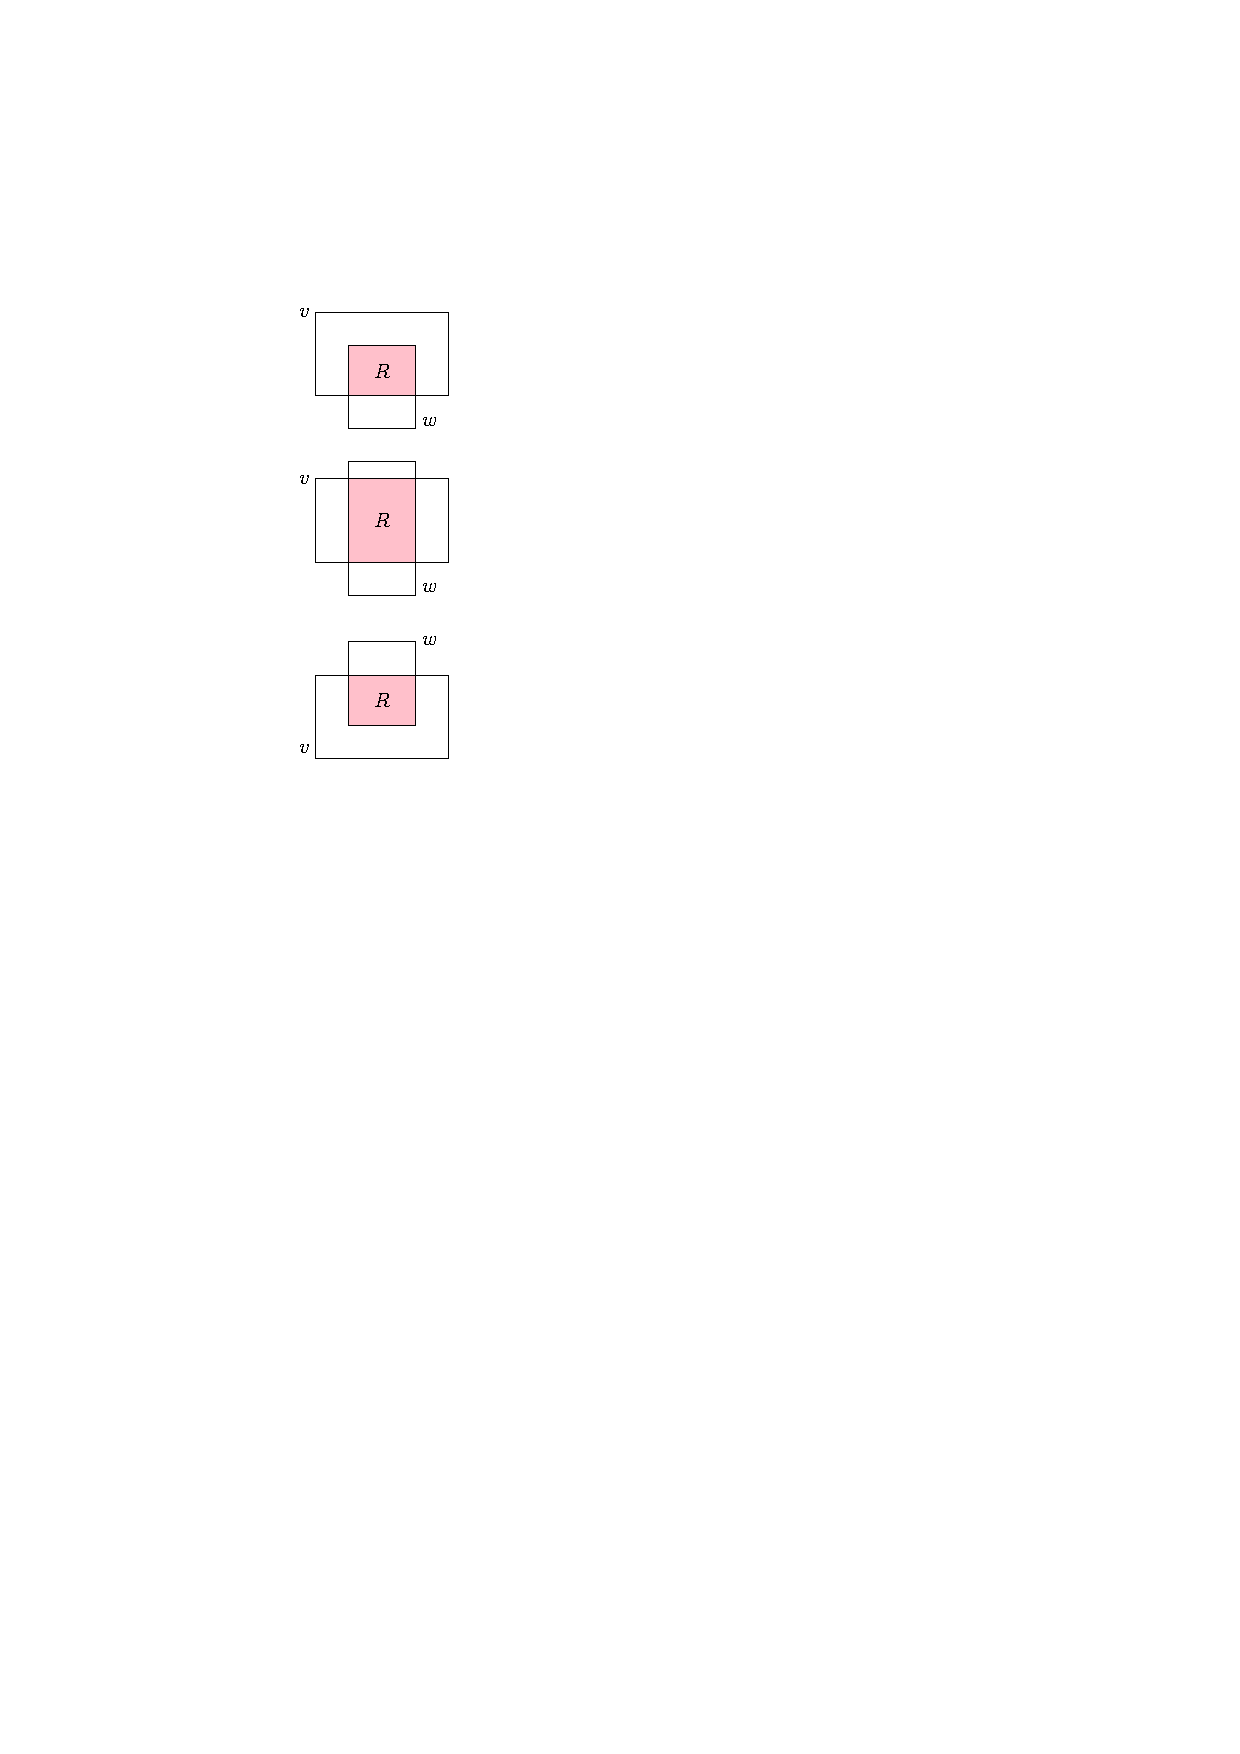
\includegraphics{figs/hvo-1} & 
   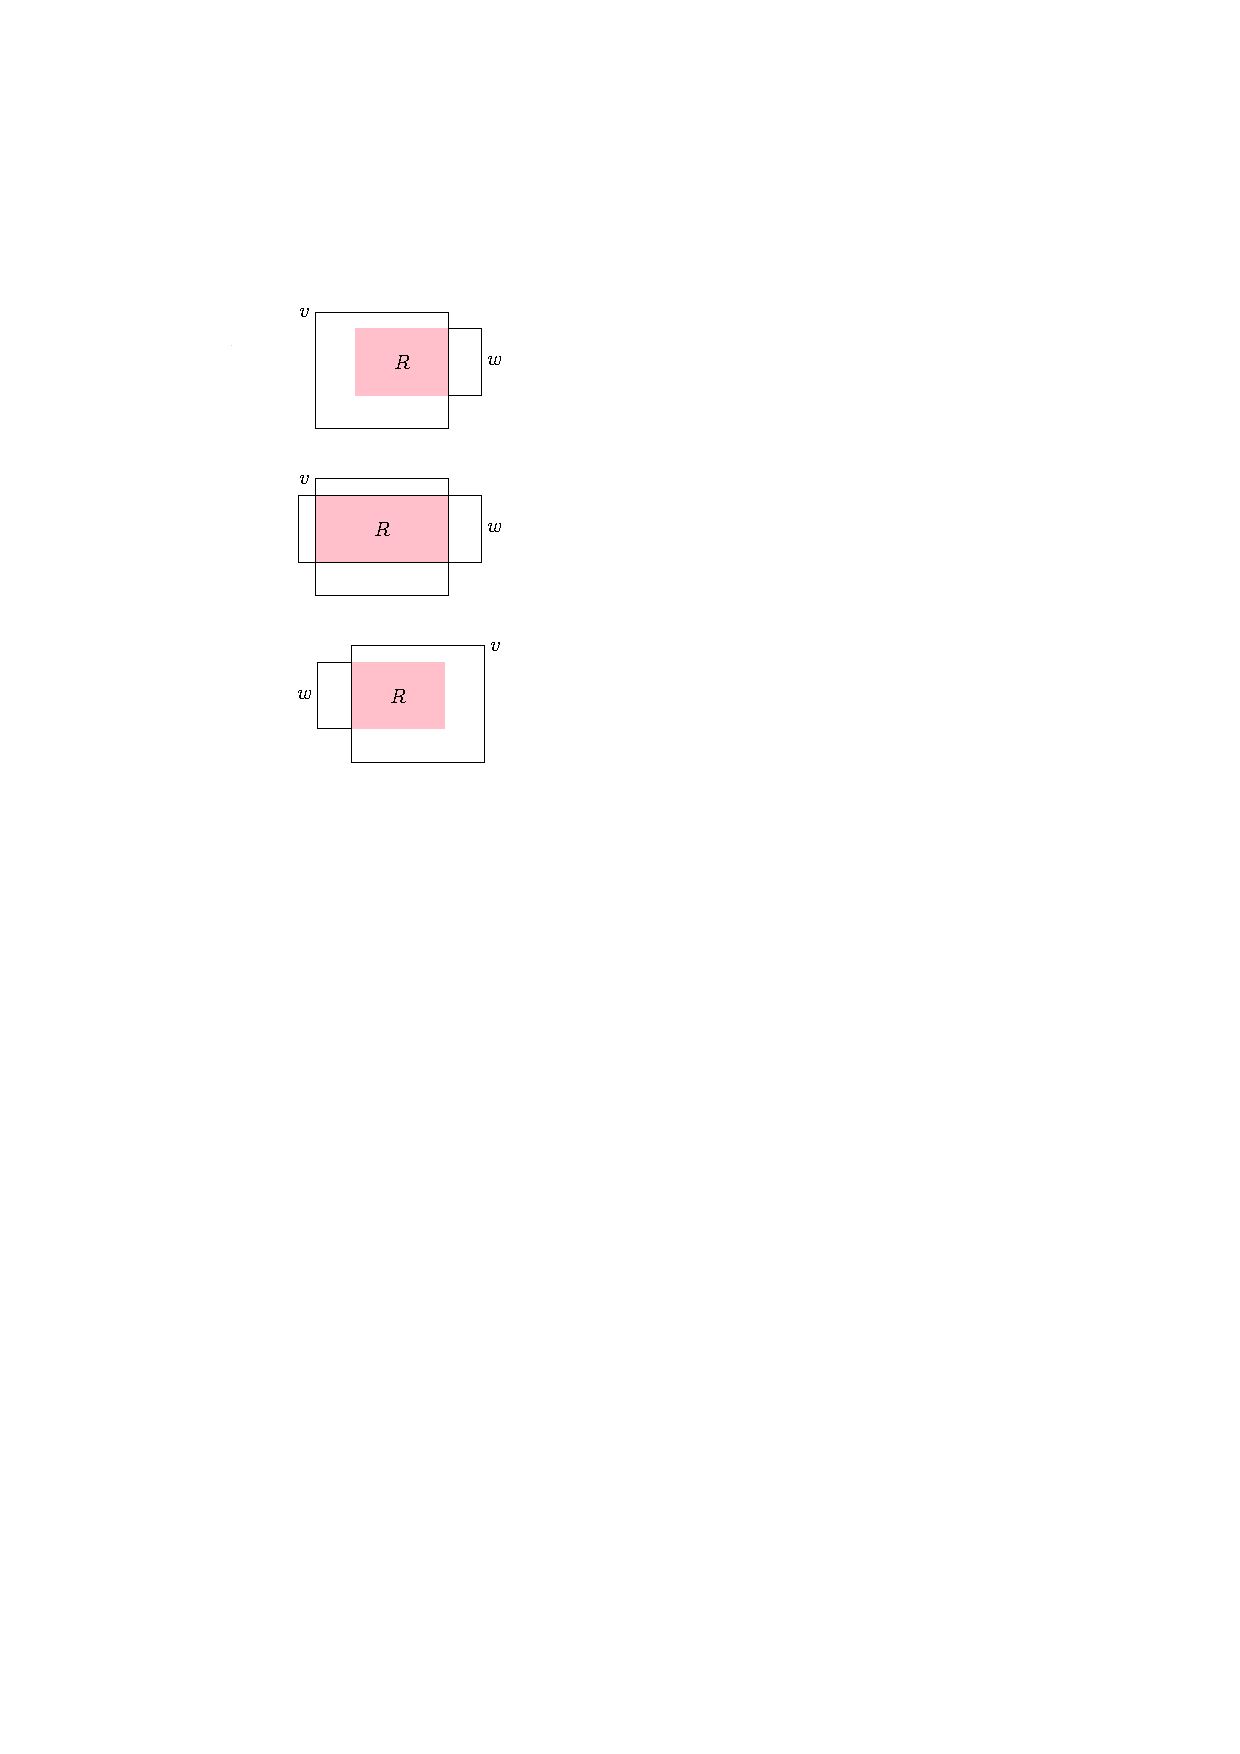
\includegraphics{figs/hvo-2} & 
   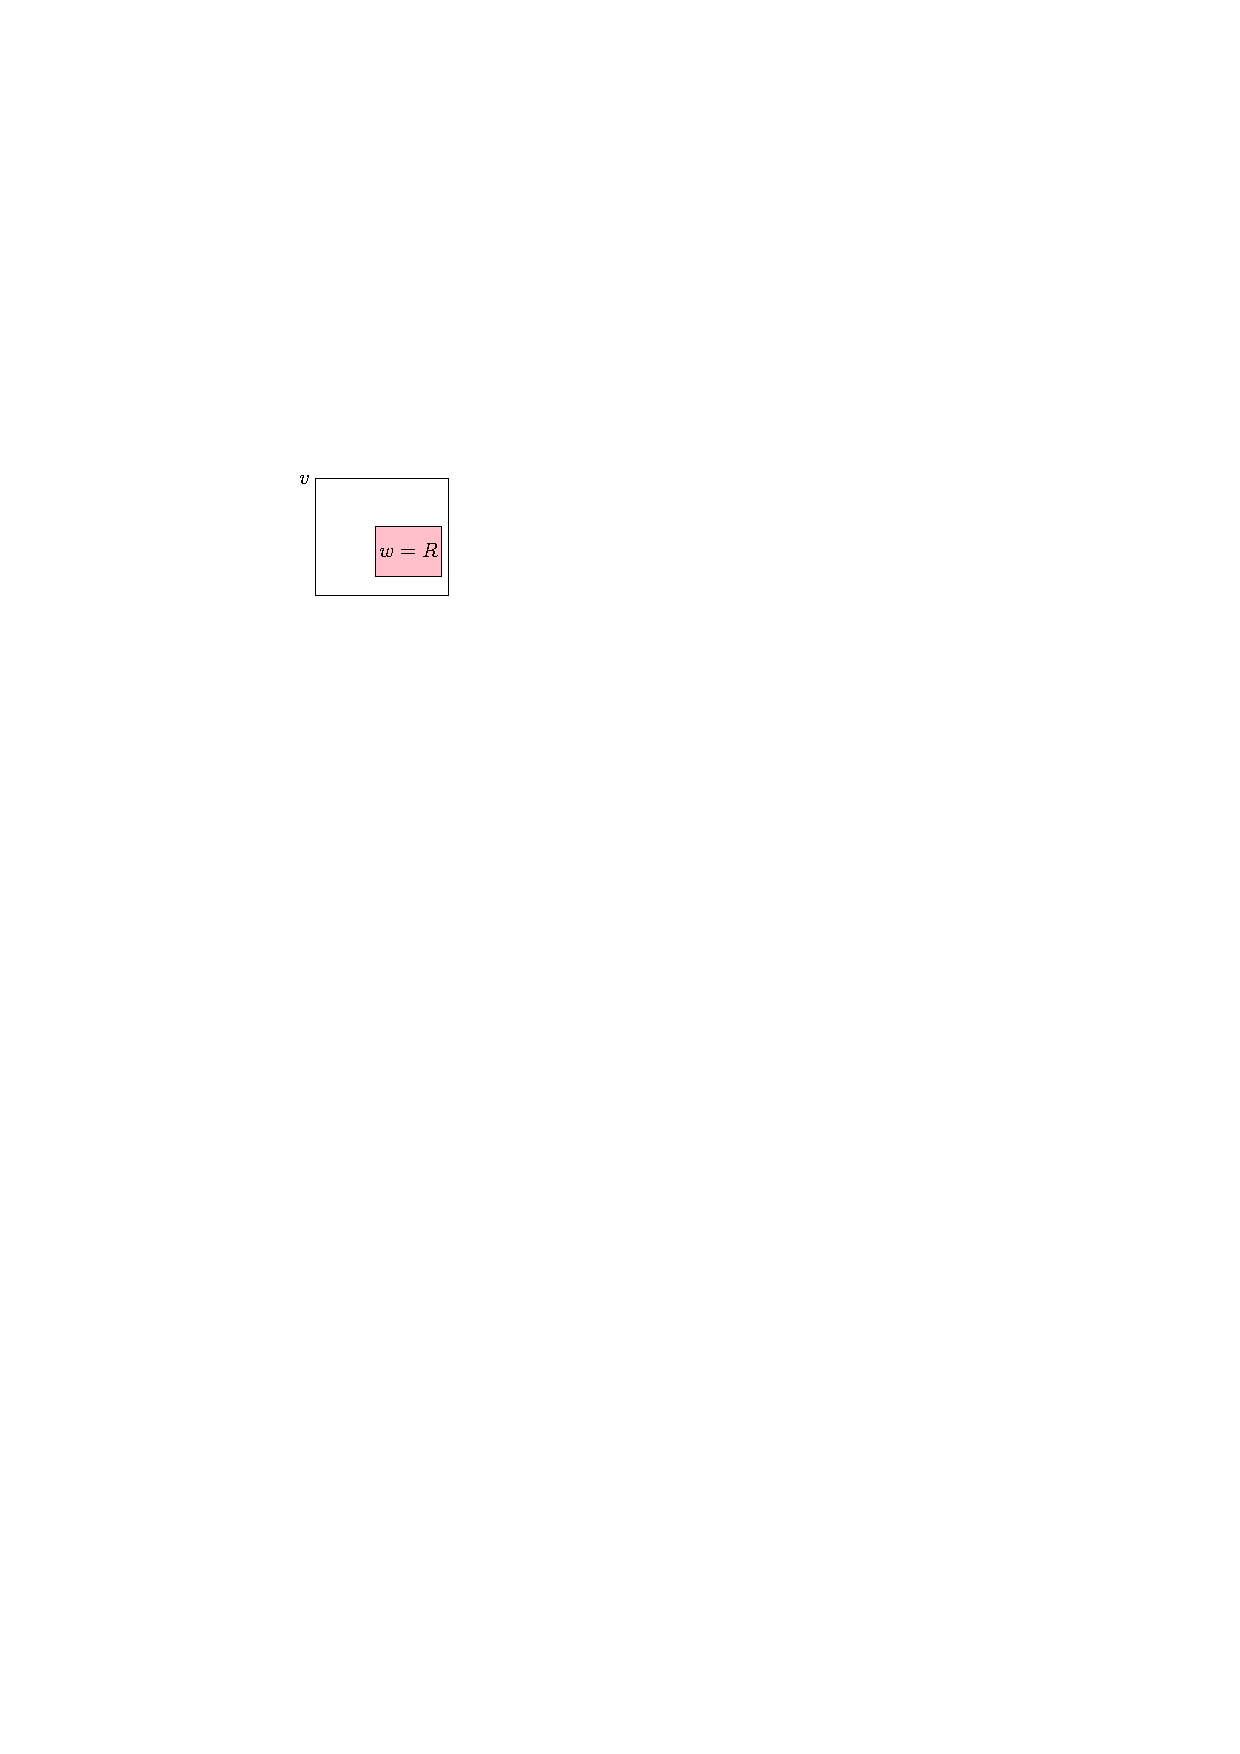
\includegraphics{figs/hvo-3} \\
   v-pairs & h-pairs & o-pair
   \end{tabular}
   \caption{Examples of v-pairs, h-pairs, and an o-pair.}
   \figlabel{hvo}
\end{figure}

Let $v_1,\ldots,v_k$ be a sequence of rectangles and let
$R_i=\bigcap_{j=1}^i v_j$.  We say that $v_1,\ldots,v_k$ is a \emph{good
sequence} if
\begin{enumerate}
  \item for each $i\in\{2,\ldots,k\}$, $v_i\cap R_{i-1}\neq \emptyset$
        and $v_i$ does not contain any corner of $R_{i-1}$; and
  \item for each $i\in\{3,\ldots,k-1\}$, $(R_{i-1},v_i)$ and
        $(R_i,v_{i+1})$ are not both h-pairs and not both v-pairs.
\end{enumerate}
See \figref{good-sequence}.

\begin{figure}
  \begin{center}
    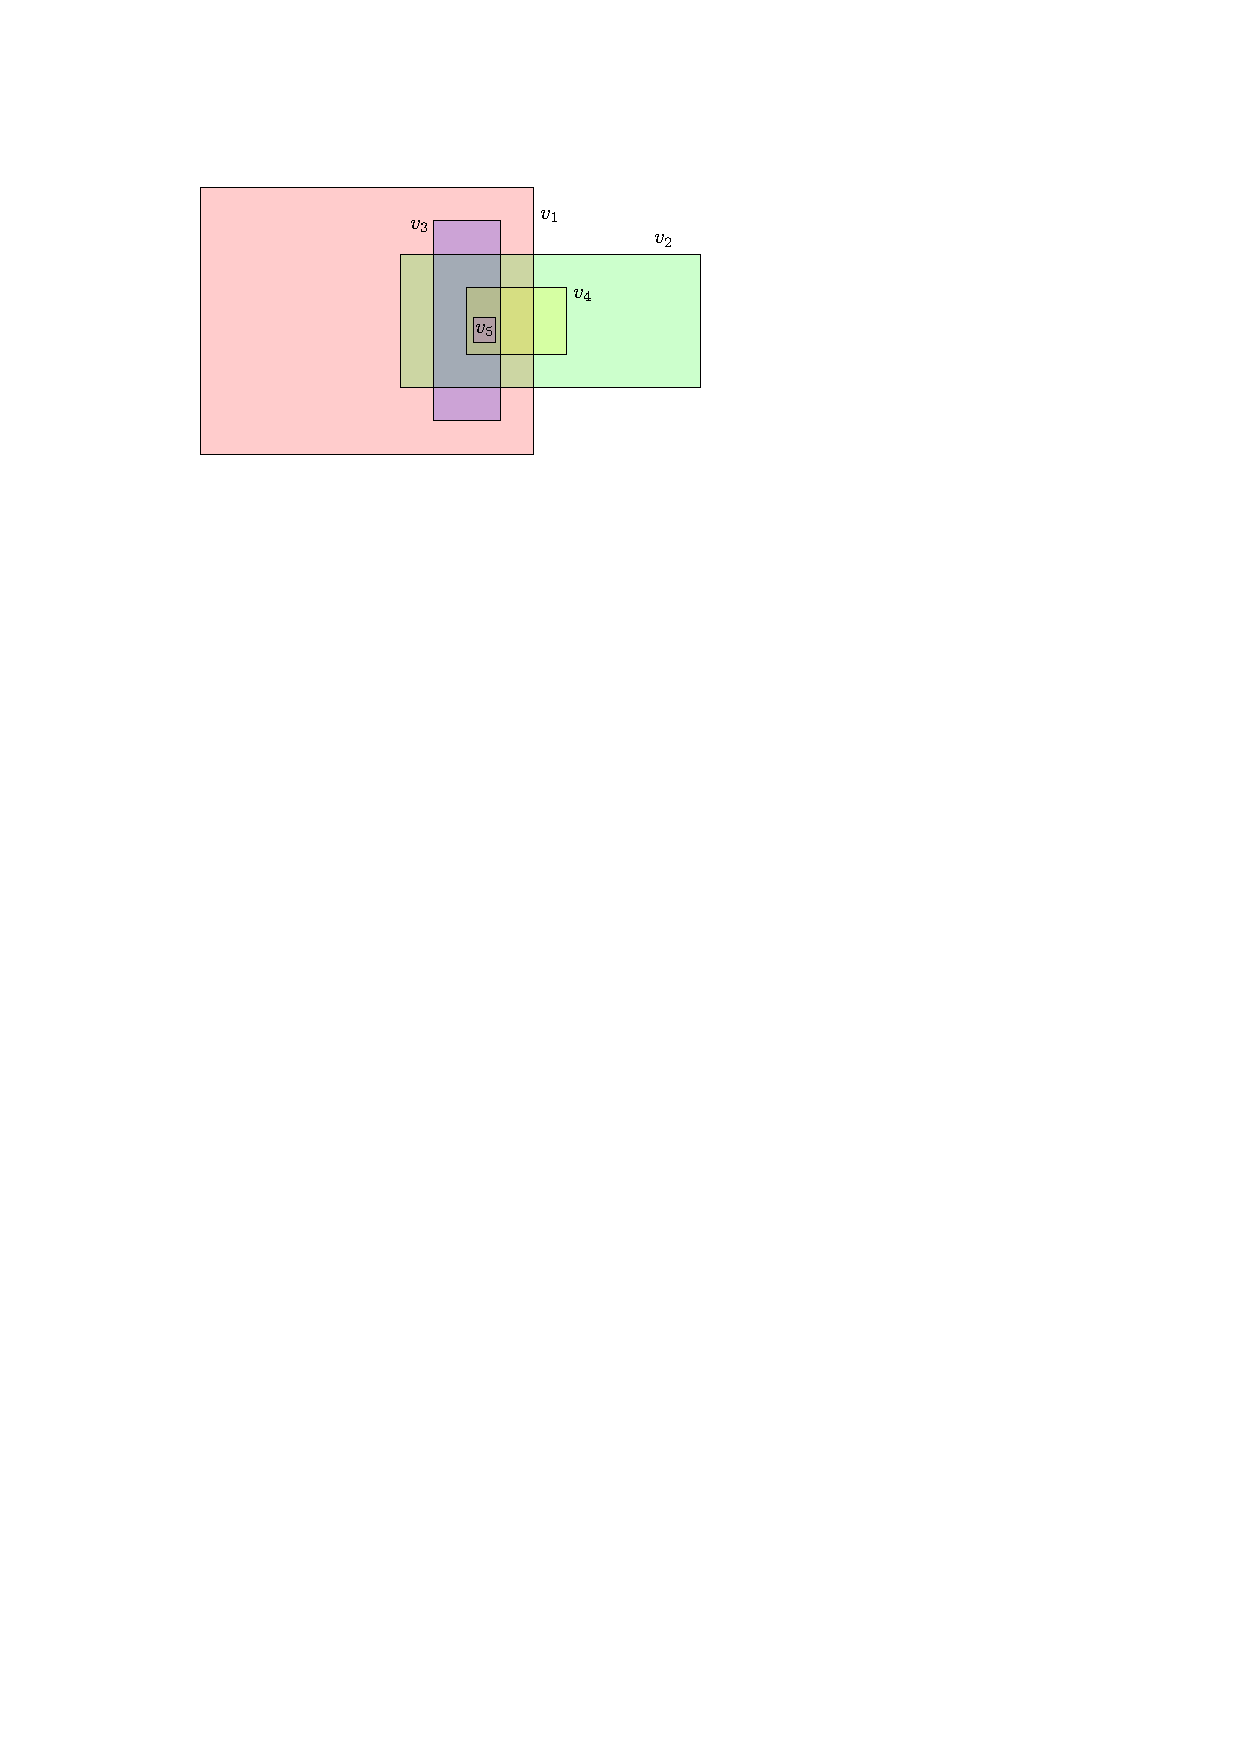
\includegraphics{figs/good-sequence}
  \end{center}
  \caption{A good sequence of rectangles.}
  \figlabel{good-sequence}
\end{figure}

We will make use of the following simple geometric lemma:
\begin{lem}\lemlabel{hv-triples}
  If $v_1,v_2,v_3$ is a good sequence of rectangles then
  $v_1\cap v_2\cap v_3=v_2\cap v_3$.
\end{lem}


\begin{proof}
  Recall that, for any two sets $A$ and $B$, $A\supseteq B$ if and only
  if $A\cap B = B$. Therefore, it is sufficient to show that $v_1\supseteq
  v_2\cap v_3$.

  If $(v_1,v_2)$ is an o-pair, then $v_1\supseteq v_2\supseteq v_2\cap
  v_3$ and we are done.  Otherwise, assume without loss of generality
  that $(R_1,v_2)=(v_1,v_2)$ is an h-pair, so that $(R_2,v_3)$ is not an
  h-pair. Refer to \figref{geometric}.  In this case, $v_2\cap v_3$ is
  contained in the rectangle $R^*$ whose top and bottom sides coincide
  with those of $v_2$ and whose left and right sides coincide with
  those of $v_1$. We finish by Observing that $v_1\supseteq R^*\supseteq
  v_2\cap v_3$, as required.
\end{proof}

\begin{figure}
  \begin{center}
    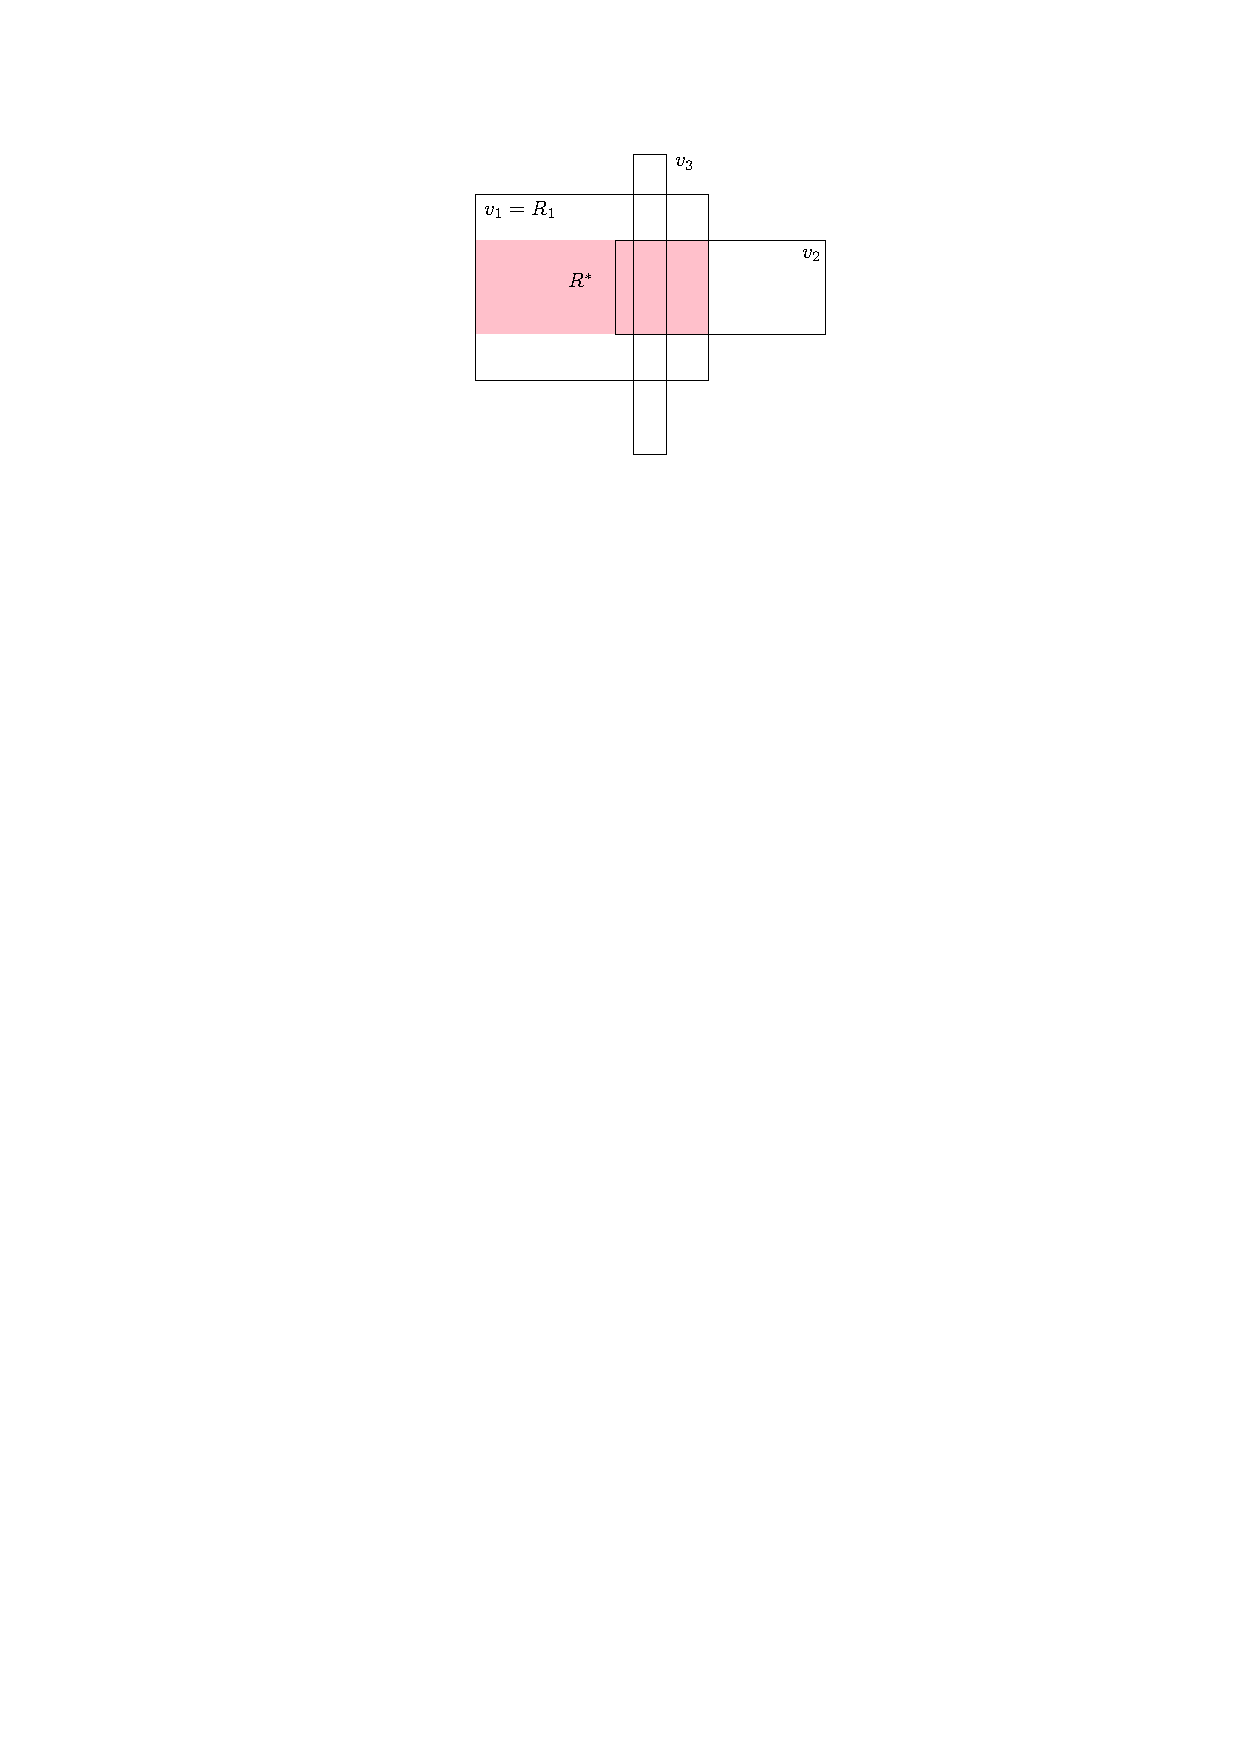
\includegraphics{figs/geometric}
  \end{center}
  \caption{The proof of \lemref{hv-triples}.}
  \figlabel{geometric}
\end{figure}


Using the transitivity of set inclusion, we obtain the following generalized
version of \lemref{hv-triples}:

\begin{cor}\corlabel{hv-sequence}
  If $v_1,\ldots,v_k$ is a good sequence of rectangles then 
  $\bigcap_{i=1}^{k} v_i = v_{k-1}\cap v_k \neq \emptyset$.
\end{cor}

A sequence $R,v_1,\ldots,v_k$ of rectangles is an \emph{h-nesting
sequence} if for each $i\in\{1,\ldots,k\}$, $(R,v_i)$ is an h-pair and,
for each $i\in\{2,\ldots,k\}$, $(R,v_{i-1}\cap v_i)$ is an h-pair.
A \emph{v-nesting sequence} is defined
similarly.
\begin{lem}
   If $R,v_1,\ldots,v_k$ is an h-nesting sequence or a v-nesting sequence,
   then there exists a point $x\in R$ such that $|\{ i: x\in v_i \}|\ge
   \lceil k/2\rceil$.
\end{lem}

\begin{proof}
   Assume, without loss of generality, that $R,v_1,\ldots,v_k$
   is an h-nesting sequence.  Consider the sequence of of
   horizontal strips $s_1,\ldots,s_k$, where each $s_i$ has top
   and bottom sides that coincide with those of $v_i$. Since each
   consecutive pair, $(v_{i-1},v_i)$, form an h-pair, $s_1\supseteq
   s_2\supseteq\cdots\supseteq s_k$.  Let $\ell$ be a point on the left
   side of $R$ contained in $s_k$ and let $r$ be a point on the right
   side of $R$ contained in $s_k$.  Since $(R,v_i)$ is a h-pair, $v_i$
   contains at least one of $\ell$ or $r$.  Therefore, at least one of
   $\ell$ or $r$ is contained in at least $\lceil k/2\rceil$ rectangles
   in $v_1,\ldots,v_k$.
\end{proof}

A \emph{rectangle intersection graph} is a graph whose vertices are
rectangles and the edge between two rectangles $u$ and $w$ is present
if and only $u\cap w\neq \emptyset$.

\subsubsection{2-Trees}


The \emph{height-$h$ $d$-branching universal 2-tree}, $T_{h,d}$ is
defined recursively as follows:
\begin{itemize}
  \item $T_{0,d}$ is the empty graph;
  \item $T_{1,d}$ is a two-vertex graph with a single edge;
  \item For $h\ge 1$, $T_{h,d}$ is obtained from $T_{h-1,d}$ by adding,
     for each edge $vw \in E(T_{i-1,d})\setminus E(T_{i-2,d})$,
     a new vertex $x_{vw}$ adjacent to both $v$ and $w$.
\end{itemize}
The \emph{root edge} of $T_{k,d}$ is the single edge of $T_{1,d}$.
The $i$-vertices of $T_{k,d}$ are \[ V_i(T_{k,d}) = V(T_{i,d}\setminus
V(T_{i-1,d}) \] and the $i$ edges of $T_{k,d}$ are \[ E_i(T_{k,d})
= E(T_{i,d}\setminus E(T_{i-1,d}) \enspace . \] For a vertex $v$ of
$T_{k,d}$, we use the notation $N_i(v)$ to denote the set of vertices
joined to $v$ by an $i$-edge.


\section{The Result}

\begin{thm}
  For each $k\in \N$, any rectangle intersection graph that contains
  $T_{4k-7,k^2}$ as a subgraph contains a clique of size $k$.
\end{thm}

\begin{proof}
  The cases $k=1$ and $k=2$ are trivial so, for the remainder of the proof
  we assume that $k\ge 2$.

  Let $G$ be a rectangle intersection graph that contains
  $T=T_{4k-7,BLAH}$ as a subgraph.  We can assume that $V(G)=V(T)$
  so that vertices of $T$ are rectangles in $V(G)$ and if vertices $v$
  and $w$ are adjacent in $T$, then $v\cap w \neq\emptyset$.

  We will attempt to define a path $v_1,\ldots,v_k$ in $T$ such that
  $v_1,\ldots,v_k$ is a good sequence of rectangles. Since every good
  sequence has  non-empty intersection, this implies that $v_1,\ldots,v_k$
  form a clique in $G$.  The only cases in which we are unable to
  complete this path occur because some point $x\in\R^2$ is contained
  in a set $X$ of $k$ vertices of $T$.  In these cases, the set $X$
  forms a $k$-clique in $G$.

  Let $vw$ be the root edge of $T$. We set $v_1=v$ and use the convention
  that $v_0=w$.  We will perform $k(k-1)$ iterations, each of which
  tries to add another vertex, $v_{i+1}$, to a partially constructed
  path $v_1,\ldots,v_i$ that forms a good sequence.  During iteration
  $t$, for each $t\in\{1,\ldots,k(k-1)\}$, the procedure will consider a
  level-$t$ vertex of $T$.  At the end of iteration $t$, the last vertex
  in the partially constructed sequence is a level-$t$ vertex.

  At the beginning of iteration $t$, $v_i$ is a level-$t$ vertex,
  so $v_{i-1}$ and $v_i$ are both adjacent to a set $S$ of $4k-7$
  level-$(t+1)$ vertices.  All the rectangles in $S$ intersect
  $R_i=\bigcup_{j=1}^i v_j$.  If all the rectangles in $S$ contain a
  corner of $R_i$, then some corner of $R_i$ is contained in at least
  \[  \left\lceil |N_{i+1}(v_i)|/4]\right\rceil 
         = \left\lceil(4k-7)/4]\right\rceil = k-1
  \]
  rectangles.  Since these rectangles are open, there is a point $x$
  contained in these $k-1$ rectangles and in $v_{i}$.  These $k$
  rectangles therefore form a $k$-clique in $G$ and we are done.

  Otherwise, some rectangle $v\in S$ does not contain a corner of $R_i$.
  Notice that the sequence $v_1,\ldots,v_i,v$ satisifies all the
  properties of a good sequence except, possibly, the pairs $(R_{i-1},v_i)$
  and $(R_i,v)$ are both h-pairs or both v-pairs.  There are two cases
  to consider:
  \begin{enumerate}
     \item $v_1,\ldots,v_i,v$ is a good sequence of rectangles. In this
       case we say that the procedure \emph{succeeds} in this iteration
       and we set $v_{i+1}=v$.

     \item  $v_1,\ldots,v_i,v$ is not a good sequence.  In this case,
       we say that the procedure \emph{stalls} in iteration $t$.  Without
       loss of generality, suppose $v_1,\ldots,v_i,v$ is not a good
       sequence because $(R_{i-1},v_i)$ and $(R_i,v)$ are both h-pairs.

       In this case, we change $v_i$ by setting $v_i=v$. We claim
       that the resulting sequence $v_1,\ldots,v_{i-1},v$ is a good
       sequence of rectangles.  To see why this is so, recall that
       $v_1,\ldots,v_{i-1}$ is a good sequence, so $(R_{i-2},v_{i-1})$
       is not an h-pair.  This means that $v_{i-2}\cap v_{i-1}
       \supseteq v_{i-1}\cap s$ where $s=(\bttom(v_i),\tp(v_i))\times
       (-\infty,\infty)$ is the horizontal strip bounded above and
       below by the top and bottom sides of $v_i$.  Since $(v_{i},v)$
       is an h-pair, $v\subseteq s$.  Therefore, $(v_{i-1},v)$ is also
       an h-pair or an o-pair and $v_1,\ldots,v_{i-1},v$ is a good sequence.

       Note that in this case we have failed to make our path any
       longer. Instead, we have only replaced the last element.
       Regardless, we continue again trying to extend the path with the
       new value of $v_i$.
  \end{enumerate}
  Notice that each iteration of the preceding two steps considers a new
  vertex, $v$, that is one level deeper in $T$ than the vertex considered
  during the previous iteration.  If we repeat these steps $k(k-1)$
  times, then one of two things occurs.
  \begin{enumerate}
     \item During these $k(k-1)$ iterations, the algorithm succeeds
     (Case~1, above) at least $k-1$ times, in which case we have
     successfully found the path $v_1,\ldots,v_k$ and whose vertices
     form a $k$-clique in $G$.

     \item During these $k(k-1)$ iterations, the algorithm stalls during
     $k$ consecutive iterations, say while trying to select $v_{i+1}$.
     During this process the vertex $v_i$ takes on $k+1$ different
     values $v_{i,0},\ldots,v_{i,k}$.  Assume, again, without loss
     of generality that $(v_{i-1},v_i)$ is an h-pair.  Then, for each
     $j\in\{0,\ldots,k-1\}$, the pair $(v_{i,j}, v_{i,j+1})$ is an h-pair,
     otherwise the procedure would have selected $v_{i,j+1}$ as $v_{i+1}$.
     This implies that the projections of $v_{i,0},\ldots,v_{i,k}$
     onto the $y$-axis are nested. (EXPLAIN BETTER)

     Furthermore, for each $j\in\{0,\ldots,k-1\}$, the pair
     $v_{i-1},v_{i,j}$ is an h-pair (and not an o-pair), otherwise the
     procedure would have succeeded in finding $v_{i+1}$ in the iteration
     immediately after $v_i$ was set to $v_{i,j}$.  This means that each
     $v_{i,0},\ldots,v_{i,k-1}$ intersects (say) the left or right side

  \end{enumerate}


  If $(v_i,v_{i+1}')$ are an o-pair, then we set $v_2=v_2'$ and continue
  as described below



   To extend the path from $v_{i-1}$ to $v_{i}$ we define
%  the set
%  \[
%     S_i = \left\{v\in N_{i}(v_{i-1})\cup N_{i+1}(v_{i-1}) : \text{$v$ contains no corner of
%           $\bigcap_{j=1}^{i-1} v_j$}\right\}
%  \]
%  We may assume that $S_i$ is non-empty because, otherwise, one of the
%  corners of $v_{i-1}$ is contained in
%  \[  \left\lceil |N_{i+1}(v_i)|/4]\right\rceil 
%      = \left\lceil(4k-7)/4]\right\rceil = k-1
%  \]
%  rectangles. Since these rectangles are open, there is a point $x$
%  contained in these $k-1$ rectangles and in $v_{i-1}$.  These $k$
%  rectangles therefore form a $k$-clique in $G$.   
%  The vertex $v_{i}$ is chosen to be some vertex in $S_i$ that
%  minimizes $\spn(v_{i-1},v_{i})$.
%
%  We claim that, for each $i\in\{2,\ldots,k\}$, $v_1,\ldots,v_i$
%  has the following properties:
% \begin{enumerate}
%    \item $v_{i}$ contains no corners of $v_{i-1}$:
%    By choice, $v_i$ intersects, but contains no corner of
%    $\bigcup_{j=1}^{i-1} v_j$. This immediately implies that $v_i$
%    contains no corner of $v_{i-1}$ (or, even any $v_j$ for $j<i$).
%
%    \item $\spn(v_{i-1},v_i)$ is minimum over all $v_i \in S_i$:  This
%    is the definition of $v_i$.
%
%    \item $\bigcap_{j=1}^i v_j = v_{i-1}\cap v_i$: For $i=2$, this is
%       immediately, so we may assume $i\ge 3$.  By induction, we may 
%       assume that $\bigcap_{j=1}^{i-1} v_j= v_{i-1}\cap v_{i-2}$.
%       We make the following two observations about $v_{i-2}$ and $v_{i-1}$:
%       \begin{enumerate}
%         \item By Property~1, above, $v_{i-2}$ contains no corner of $v_{i-1}$.
%         \item Since $v_{i-2}$ and $v_{i-1}$ are joined by an edge in $T$,
%       $v_{j-1}\cap v_{j-2}\neq\emptyset$.  
%       \end{enumerate}
%       These two observations imply that
%       the rectangle $R=\v_{j-1}\cap v_{j-2}$ has two edges that are
%       contained in $\partial v_{j-1}$ and at most two edges that are
%       contained in $\partial v_{j-2}$.  We claim that $v_j
%
% (Property~1, above)
%       and $v_{
%
%
%=v_{j}$
%
%    \item FIXME: Unnecessary.  $\bigcap_{j=1}^i v_j \neq\emptyset$: For $i=2$, this follows
%    immediately from the fact that $v_1$ and $v_2$ are joined by an edge
%    in $T$, so we may assume that $i\ge 3$.
%
%    By the definitions of $S_i$ and $T$, the edges $v_{i-1}v_i$
%    and $v_{i-2}v_i$ are both in $T$, so that $v_i\cap v_{i-1}\cap
%    v_{i-2}\neq \emptyset$.  Since $v_1,\ldots,v_{i-1}$ has Property~3,
%    $v_{i-1}\cap v_{i-2}=\bigcap_{j=1}^{i-1} v_j$, so
%    \[
%       \bigcap_{j=1}^i v_j = v_i\cap v_{i-1}\cap v_{i-2} \neq \emptyset 
%         \enspace .
%    \]
%  \end{enumerate}
%  This completes the proof of the theorem, since the final property implies
%  that $v_1,\ldots,v_k$ form a $k$-clique in $G$.
\end{proof}



\bibliography{op}
\bibliographystyle{plainurl}
\end{document}
